%%% SETUP %%%%%%%%%%%%%%%%%%%%%%%%%%%%%%%%%%%%%%%%%%%%%%%%%%%%%%%%%%%%%%%%%%%%%%

%%% DOCUMENT TYPE %%%%%%%%%%%%%%%%%%%%%%%%%%%%%%%%%%%%%%%%%%%%%%%%%%%%%%%%%%%%%%

\documentclass[10pt,twocolumn, a4paper]{article}

%%% PACKAGES %%%%%%%%%%%%%%%%%%%%%%%%%%%%%%%%%%%%%%%%%%%%%%%%%%%%%%%%%%%%%%%%%%%

% Encoding

\usepackage[utf8]{inputenc}
\usepackage[T1]{fontenc}

% Geometry
\usepackage{multirow}
\usepackage{graphicx}
\usepackage{geometry} % edit margins of paper
\usepackage{setspace} % edit line spacing
\usepackage{fancyhdr} % header, footer
\usepackage{titlesec} % edit format of titles

% Visual

\usepackage[dvipsnames]{xcolor} % colors
\usepackage{tikz} % graphics
\usepackage[framemethod=tikz]{mdframed} % frames, better theorems

% Math

\usepackage{amsmath} % math tools
\usepackage{amssymb} % math symbols
\usepackage{amsthm} % thereoms
\usepackage{mathtools} % math tools

% Referencing

\usepackage{nameref}
\usepackage{hyperref}
\usepackage{cleveref}
% Useful

\usepackage[shortlabels]{enumitem} % enumerations

% Other

\usepackage{lastpage} % get number of last page

%%% MARGINS %%%%%%%%%%%%%%%%%%%%%%%%%%%%%%%%%%%%%%%%%%%%%%%%%%%%%%%%%%%%%%%%%%%%

\geometry{a4paper, left=20mm, right=20mm, top=20mm, bottom=20mm, includehead}

%%% COLORS %%%%%%%%%%%%%%%%%%%%%%%%%%%%%%%%%%%%%%%%%%%%%%%%%%%%%%%%%%%%%%%%%%%%%

%%% TITLES %%%%%%%%%%%%%%%%%%%%%%%%%%%%%%%%%%%%%%%%%%%%%%%%%%%%%%%%%%%%%%%%%%%%%

\colorlet{color-section}                {BrickRed}
\colorlet{color-subsection}             {BrickRed}

%%% MATH BOXES %%%%%%%%%%%%%%%%%%%%%%%%%%%%%%%%%%%%%%%%%%%%%%%%%%%%%%%%%%%%%%%%%

\colorlet{color-definition}             {SpringGreen!20}
\colorlet{color-theorem}                {Apricot!13}
\colorlet{color-proposition}            {Apricot!13}
\colorlet{color-corollary}              {Apricot!13}
\colorlet{color-lemma}                  {Apricot!13}
\colorlet{color-remark}                 {Gray!5}
\colorlet{color-example}                {Lavender!7}
% \colorlet{color-proof}                  {FILL COLOR HERE}


%%% CAPTIONS %%%%%%%%%%%%%%%%%%%%%%%%%%%%%%%%%%%%%%%%%%%%%%%%%%%%%%%%%%%%%%%%%%%

%%% CAPTION DEFINITION %%%%%%%%%%%%%%%%%%%%%%%%%%%%%%%%%%%%%%%%%%%%%%%%%%%%%%%%%

\newcommand*{\definitionname}{Definition}
\newcommand*{\theoremname}{Theorem}
\newcommand*{\propositionname}{Proposition}
\newcommand*{\corollaryname}{Corollary}
\newcommand*{\lemmaname}{Lemma}
\newcommand*{\remarkname}{Remark}
\newcommand*{\examplename}{Example}


%%% SHORTCUTS %%%%%%%%%%%%%%%%%%%%%%%%%%%%%%%%%%%%%%%%%%%%%%%%%%%%%%%%%%%%%%%%%%

%%% SINGLE SYMBOLS %%%%%%%%%%%%%%%%%%%%%%%%%%%%%%%%%%%%%%%%%%%%%%%%%%%%%%%%%%%%

% Logic

% \forall exists
% \exists exists
% \lnot exists
% \lor exists
% \land exists
\newcommand*{\limp}{\rightarrow}
\newcommand*{\limps}{\; \limp \;} % \limp with some space around
\newcommand*{\leqv}{\leftrightarrow}
\newcommand*{\leqvs}{\; \leqvs \;} % \leqv with some space around

% Meta Logic

% \implies exists
% \iff exists

% Colon Stuff

\newcommand*{\cl}{\colon}
\newcommand*{\cleq}{\coloneqq}
\newcommand*{\eqcl}{\eqqcolon}

% Sets

\newcommand*{\N}{\mathbb{N}} % natural numbers
\newcommand*{\Z}{\mathbb{Z}} % integers
\newcommand*{\Q}{\mathbb{Q}} % rational numbers
\newcommand*{\R}{\mathbb{R}} % real numbers
\newcommand*{\C}{\mathbb{C}} % complex numbers

%%% MATH OPERATORS %%%%%%%%%%%%%%%%%%%%%%%%%%%%%%%%%%%%%%%%%%%%%%%%%%%%%%%%%%%%%

% General

\DeclareMathOperator{\id}{id}
\DeclareMathOperator{\sgn}{sgn}

%%% TEMPLATES %%%%%%%%%%%%%%%%%%%%%%%%%%%%%%%%%%%%%%%%%%%%%%%%%%%%%%%%%%%%%%%%%%

% General

% write a set definition like: { #1 | #2 }
\newcommand*{\setdefinition}[2]{
  \left\{ #1 \mathrel{}\middle|\mathrel{} #2 \right\}
}

% write a nice map definition
\newcommand*{\mapdefinition}[5]{
  \begin{align*}
    #1 \cl #2 &\to     #3 \\
           #4 &\mapsto #5
  \end{align*}
}


%%% FORMATTING %%%%%%%%%%%%%%%%%%%%%%%%%%%%%%%%%%%%%%%%%%%%%%%%%%%%%%%%%%%%%%%%%

%%% HEADER, FOOTER %%%%%%%%%%%%%%%%%%%%%%%%%%%%%%%%%%%%%%%%%%%%%%%%%%%%%%%%%%%%%

\pagestyle{fancy}
\fancyhf{} % clear everything
\lhead{\sffamily}
\chead{\sffamily \large \bfseries Tichu strategies depending on course of play}
\rhead{\sffamily Page \thepage /\pageref*{LastPage}}
\lfoot{}
\cfoot{}
\rfoot{}

%%% TITLE FORMAT %%%%%%%%%%%%%%%%%%%%%%%%%%%%%%%%%%%%%%%%%%%%%%%%%%%%%%%%%%%%%%%

\setcounter{secnumdepth}{2}

\titleformat{\chapter}[display]
{\normalfont\huge\bfseries}{\chaptertitlename\ \thechapter}{20pt}{\Huge}
\titleformat{\section}[frame]
{\normalfont\LARGE\bfseries\color{color-section}\scshape}{\filright\,\thesection\,}{0.2ex}{\filcenter}
\titleformat{\subsection}
{\normalfont\Large\bfseries\color{color-subsection}}{\thesubsection}{1em}{}
\titleformat{\subsubsection}
{\normalfont\normalsize\bfseries}{\thesubsubsection}{1em}{}
\titleformat{\paragraph}[runin]
{\normalfont\normalsize\bfseries}{\theparagraph}{1em}{}
\titleformat{\subparagraph}[runin]
{\normalfont\normalsize\bfseries}{\thesubparagraph}{1em}{}

%%% SPACING %%%%%%%%%%%%%%%%%%%%%%%%%%%%%%%%%%%%%%%%%%%%%%%%%%%%%%%%%%%%%%

% Titles

\titlespacing*{\chapter}{0pt}{50pt}{40pt}
\titlespacing*{\section}{0pt}{3.5ex plus 1ex minus .2ex}{2.3ex plus .2ex}
\titlespacing*{\subsection}{0pt}{3.25ex plus 1ex minus .2ex}{1.5ex plus .2ex}
\titlespacing*{\subsubsection}{0pt}{3.25ex plus 1ex minus .2ex}{1.5ex plus .2ex}
\titlespacing*{\paragraph}{0pt}{3.25ex plus 1ex minus .2ex}{1em}
\titlespacing*{\subparagraph}{\parindent}{3.25ex plus 1ex minus .2ex}{1em}

% Text, Paragraphs

%\setstretch{1.05} % scaling of space between lines
\setlength{\parindent}{0pt} % indentation of paragraphs
%\setlength{\parskip}{4.0pt plus 1.0pt minus 1.0pt} % space between paragraphs
\setlength{\parskip}{0.8ex}
\setlength{\topsep}{0pt}

%%% SYMBOLS USED BY NUMBERINGS, ENVIRONMENTS, ... %%%%%%%%%%%%%%%%%%%%%%%%%%%%%%

% \renewcommand*\qedsymbol{$\blacksquare$} % alternative QED symbol
\renewcommand{\thefootnote}{\arabic{footnote}} % normal footnotes on page
\renewcommand{\thempfootnote}{\fnsymbol{mpfootnote}} % footnotes on minipages, e.g. in mdframed environments

%%% LISTS, ENUMERATIONS %%%%%%%%%%%%%%%%%%%%%%%%%%%%%%%%%%%%%%%%%%%%%%%%%%%%%%%%

% 'itemize'

\setlist[itemize]{noitemsep, topsep=0pt}

% 'enumerate'

% no special settings at the moment

% 'description'

% no special settings at the moment

% 'axioms'

\newlist{axioms}{enumerate}{2}
\setlist[axioms]{itemsep=0pt,label*=\arabic*.}

%%% MDFRAMED PATCH %%%%%%%%%%%%%%%%%%%%%%%%%%%%%%%%%%%%%%%%%%%%%%%%%%%%%%%%%%%%%

\usepackage{xpatch}

\makeatletter
\xpatchcmd{\endmdframed}
  {\aftergroup\endmdf@trivlist\color@endgroup}
  {\endmdf@trivlist\color@endgroup\@doendpe}
  {}{}
\makeatother

%%% MDFRAMED STYLES %%%%%%%%%%%%%%%%%%%%%%%%%%%%%%%%%%%%%%%%%%%%%%%%%%%%%%%%%%%%

% thick frame and bar for title

\mdfdefinestyle{style-box}{
  skipabove=1.5ex plus .5ex minus .2ex,
  skipbelow=1ex plus .2ex minus .2ex,
  linewidth=2pt,
  linecolor=Gray!20,
%   roundcorner=3pt,
  innerleftmargin=0.5\baselineskip,
  innerrightmargin=0.5\baselineskip,
  innertopmargin=0.4\baselineskip,
  innerbottommargin=0.4\baselineskip,
  frametitlebackgroundcolor=Gray!20,
  frametitleaboveskip=0.3pt,
  frametitlebelowskip=0.3pt,
  theoremseparator=,
  theoremspace=\hfill,
  theoremtitlefont=\mdseries\scshape,
  nobreak=true
}

% highlighted background

\mdfdefinestyle{style-background}{
  skipabove=1.5ex plus .5ex minus .2ex,
  skipbelow=1ex plus .2ex minus .2ex,
  hidealllines=true,
  backgroundcolor=Gray!5,
  innerleftmargin=0.5\baselineskip,
  innerrightmargin=0.5\baselineskip,
  innertopmargin=0.4\baselineskip,
  innerbottommargin=0.4\baselineskip,
}

% thin frame

\mdfdefinestyle{style-leftline}{
  skipabove=1.5ex plus .5ex minus .2ex,
  skipbelow=1ex plus .2ex minus .2ex,
  linewidth=1pt,
  linecolor=Gray!50,
  topline=false,
  bottomline=false,
  rightline=false,
  innerleftmargin=0.5\baselineskip,
  innerrightmargin=0,
  innertopmargin=0.2\baselineskip,
  innerbottommargin=0.0\baselineskip,
}

%%% ENVIRONMENTS %%%%%%%%%%%%%%%%%%%%%%%%%%%%%%%%%%%%%%%%%%%%%%%%%%%%%%%%%%%%%%%

% Definition

\mdtheorem[
  style=style-box,
  linecolor=color-definition,
  frametitlebackgroundcolor=color-definition
]{definition}{\definitionname}[section]

% Theorem

\mdtheorem[
  style=style-box,
  linecolor=color-theorem,
  frametitlebackgroundcolor=color-theorem,
  font=\itshape
]{theorem}{\theoremname}[section]

% Proposition

\mdtheorem[
  style=style-box,
  linecolor=color-proposition,
  frametitlebackgroundcolor=color-proposition,
  font=\itshape
]{proposition}[theorem]{\propositionname}

% Corollary

\mdtheorem[
  style=style-box,
  linecolor=color-corollary,
  frametitlebackgroundcolor=color-corollary,
  font=\itshape
]{corollary}[theorem]{\corollaryname}

% Lemma

\mdtheorem[
  style=style-box,
  linecolor=color-lemma,
  frametitlebackgroundcolor=color-lemma,
  font=\itshape
]{lemma}[theorem]{\lemmaname}

\theoremstyle{remark}

% Remark

\newtheorem*{remark}{\remarkname}
\surroundwithmdframed[
  style=style-background,
  backgroundcolor=color-remark
]{remark}

% Example

\newtheorem*{example}{\examplename}
\surroundwithmdframed[
  style=style-background,
  backgroundcolor=color-example
]{example}

% Proof

\surroundwithmdframed[
  style=style-leftline
]{proof}

%%% TEXT FORMATTING %%%%%%%%%%%%%%%%%%%%%%%%%%%%%%%%%%%%%%%%%%%%%%%%%%%%%%%%%%%%

% definitions

\newcommand*{\df}[1]{\textbf{#1}}



%%% LANGUAGE %%%%%%%%%%%%%%%%%%%%%%%%%%%%%%%%%%%%%%%%%%%%%%%%%%%%%%%%%%%%%%%%%%%

%%% SETUP %%%%%%%%%%%%%%%%%%%%%%%%%%%%%%%%%%%%%%%%%%%%%%%%%%%%%%%%%%%%%%%%%%%%%%

\usepackage[english]{babel}

%%% CAPTION REDEFINITION %%%%%%%%%%%%%%%%%%%%%%%%%%%%%%%%%%%%%%%%%%%%%%%%%%%%%%%



%%% HYPHENATION %%%%%%%%%%%%%%%%%%%%%%%%%%%%%%%%%%%%%%%%%%%%%%%%%%%%%%%%%%%%%%%%




%%% DOCUMENT %%%%%%%%%%%%%%%%%%%%%%%%%%%%%%%%%%%%%%%%%%%%%%%%%%%%%%%%%%%%%%%%%%%
%\usepackage{slashbox}
\usepackage{multirow}
\usepackage{listings}

\begin{document}

\title{Tichu strategies depending on course of play}
\date{June 03, 2020}
\author{Matthias Schmickler \and Paul Sander \and Jean-Luc Portner \and Tom Haidinger \and Andrey Bryutkin \\ \\ Swiss Federal Institute of Technology Zurich (ETH)}
\maketitle

\section{Motivation and goals}

A prevalent characteristic of both mathematics and physics is their elaborate structure of interdependent concepts. It is only natural, then, for us students to thrive off of complexity and intricateness both within our courses as well as throughout our daily life. One such endeavour we satisfy our free time with is the game of Tichu. Tichu is a team card game taught to us by older students of our courses during the, albeit not very wide-ranging, cultural melting-pot between years – that unproductive period when our courses’ study hall slowly turns into the Mensa. 

    In addition to luck and strategy, this game became popular within our friend-group due to its fairly unique aspect of interaction. Allowing for multiple possible card combinations, special cards and a process of card switching, Tichu derives its complexity not through complicated rules, but rather through diverseness of strategy. Indeed, given one must adapt to one’s opponents’ and teammate’s strategies, one may say its strategies are interactive and reactive in nature. Therefore – although we note that card games are hard to analyse in general – we believe Tichu is indeed approachable through game-theoretic methods. 

    Fascinated by this type of game and equipped with tools from our game theory course, we pose the general question: “which strategy should we pursue as players?”. We shall further differentiate this admittedly vague question into: “what strategy should we pursue given”: a) “we know what player-type all other players are” and b) “we do not know anything about other players”. 
\section{Introduction on Tichu}

Tichu is a complicated team card game with many rounds that will be explained in detail below. The gist of it is that a set of playing cards is distributed among four players, two of which form a team, and card combinations are played to trump each other and win cards that score different amounts of points. At the beginning of each round each player exchanges a card with every other player, influencing the player dynamics of each round. Additionally, a bet, called a Tichu, can be placed on exiting a round of the game first, which yields bonus points. Teams then fight to reach 1000 points first. Obviously, this is not a full explanation, rather it serves to highlight the most important aspects of the game and subsequently the most interesting mechanisms explored in this essay, namely: the exchange stage, the player dynamics and the betting mechanism of a Tichu. 

A game of Tichu consists of two teams with two players each. The game is divided into multiple rounds that host opportunities to score and even lose points. The game ends when one team has collected 1000 or more points. In every round of the game each player is dealt 14 cards from the 56-card deck. To begin a round, each player must exchange one card with every other player; we coin this game mechanism the ‘exchange stage’. Points can be scored through:\\
\begin{enumerate}
\item claiming specific cards with point values
\item announcing a Tichu (a bet)
\item performing a double win
\end{enumerate}

A round begins when the player with the Mah Jong card in his deck (explained later) plays a valid card combination or singleton. The other players can play higher variations of strictly the same card combination-type to trump the previously played cards. A play continues until all other players are unable or unwilling to trump (they may choose to pass) the current card combination. Then, the winning player ‘claims’ the played cards and may start the next play. ‘Exiting’ a round refers to a player having played all of his 14 cards. A round ends when two players from the same team exit the round.


A Tichu card set consists of the cards: 2, 3, 4, 5, 6, 7, 8, 9, 10, J, Q, K, A in four different colours: black, blue, green and red. Additionally, four special cards include the: Dragon, Phoenix, Dog and Mah Jong (explored later). Only a few cards have specific values:\\
\begin{scriptsize}
\begin{center}
\begin{tabular}{ c c c }
\textbf{5} & $\sim$  & \textbf{5 P} \\
\textbf{10} & $\sim$ & \textbf{10 P} \\
\textbf{K} & $\sim$  & \textbf{10 P} \\
\textbf{Dragon} & $\sim$ & \textbf{25 P} \\
\textbf{Phoenix} & $\sim$ & \textbf{-25 P}
\end{tabular}
\end{center}
\end{scriptsize}
In total a round distributes 100 points among both teams, however it is theoretically possible to end a round with a 125:-25 team point distribution as the Dragon and Phoenix cards respectively incur a win or loss of 25 points.

Here are several valid card combinations:
\\
\\
\resizebox{0.5\textwidth}{!}{%
\begin{tabular}{ c c c }
\textbf{High Card} & $\sim$  & \textbf{2 $<$ 3 $< ... <$ A} \\
\textbf{Pair} & $\sim$ & \textbf{(2,2) $< ... <$ (A,A)} \\
\textbf{Triple} & $\sim$  & \textbf{(2,2,2) $< ... <$ (A,A,A)} \\
\textbf{Following Pairs} & $\sim$ &  \textbf{(2,2,3,3, ...) $< ... < $ (..., K,K,A,A)}
 \\
\textbf{Full House} & $\sim$ &  \textbf{(2,2,2,A,A) $<... <$ (A,A,A,K,K)} \\
\textbf{Street(more than 5 cards)} & $\sim$ & \textbf{(2,3,4,5,6, ...) $< ... < $(...,10,J,Q,K,A)}
\end{tabular}%
}

These combinations can only be trumped through higher variations of strictly the same combination-type. Exempt from this rule are ‘Bombs’. Bombs can be played at any point during a round, even if it is not that player’s turn, and only yield only too higher or equal variations of itself. Bombs consist of four of a kind cards, while Street Bombs consist of single-colour streets and are stronger. As with normal Streets, Street Bombs are stronger the more cards they consist of:
\\
\\
\resizebox{0.5\textwidth}{!}{%
\begin{tabular}{ c c c }
\textbf{Bomb} & $\sim$  & \textbf{(2,2,2,2), $< ... <$ (A,A,A,A)} \\
\textbf{Street Bomb} & $\sim$ & \textbf{(A,A,A,A) $<$ (2,3,4,5,6) $<$ (2,3,4,5,6, ...) $< ... < $ (...,10,J,Q,K,A)} \\ \\
\end{tabular}%
}

\paragraph*{Mah Jong}
The player with this card in his deck starts the game. Mah Jong may be played as a \textbf{1} High Card or combined into a Street. Additionally, the player may request a non-special card to be played. This card must be played immediately at the next possible legal opportunity by any player.
\paragraph*{Dog}
Playing this card transfers the right to begin a play to the player’s teammate. If this teammate has already exited the round, the next active player inherits this right. It cannot be played in any combination.
\paragraph*{Phoenix}
The Phoenix acts as a Joker and can substitute any non-special card and be played in any combination. Played as a singleton it counts as +0.5 of any card it trumps, excluding special cards like the Dragon.
\paragraph{Dragon}
The Dragon is the highest possible singleton available and trumps the Phoenix card. The cards claimed for any play won through this card must be awarded to either opponent. The Dragon may only be bombed, in this case the new winner can claim the cards and must not award them to either opponent.

Special cards cannot be played in any type of Bomb.

At the end of a round, after two teammates have managed to exit, either one or both opponents have not exited the round. If one opponent remains, both his claimed cards and his remaining hand cards are gifted to the player that exited the round first. All other claimed cards are valued based on their worth as listed above and added to the team score. On the other hand, if two teammates manage to exit before both opponents, the value of claimed cards is disregarded completely and 200 points are immediately awarded to the winning team; this is called a double win.

Finally, a Tichu is a 100 point bet a player takes on exiting the round first. Success scores an additional 100 points while failure incurs a cost of 100 points. A Tichu can be announced as long as the player has not played any cards yet. Similarly, a Grand Tichu is a bet of 200 points and must be announced after the 8th card is dealt. A Grand Tichu may therefore also have an impact on the Exchange stage.

For the following discussion we would like to coin ‘good’ cards, in contrast to ‘bad’ cards, as cards that allow for strong combinations and possibly multiple different strong actions throughout the development of the round.


\section{Our Model and approximations}
\subsection{Basic assumptions}
Our basic approximation consists of two distinctions regarding player behavior and transparency of information. 

In our consideration we would like to define the following two types of players.
The first player is the "aggressive player" - he is characterized by the fact that he takes a higher risk and pays more attention to the value of his cards and less to his playing partner. In case of doubt he will keep the good cards and give his partner something worse than the other way round.
The willingness to take risks is characterized by the fact that even with below average cards (relative to cards with which the average player would announce a tichu) he already announces the tichu. 

The second player is the "defensive player". This stands in contrast to the "aggressive player type". He is rather risk-averse, which means he needs above average (relative to cards with which the average player would announce a tichu) good cards to announce a tichu.
When exchanging cards he decides to give the good card to his partner instead of keeping it himself.

To make it easier to identify the players in the following, the following notation is introduced:
We will store information on the players behaviour in a vector $\alpha \in \{0,1\}^4$.
\\ 
\begin{itemize}
\item A: "aggressive player" will be assigned to $\alpha_i = 1$
\item D: "defensive player" will be assigned to $\alpha_i = 0$ \\
\end{itemize} 
In our approximation of Tichu, we consider two possible situations. 
The first situation is characterized by transparency. Every player knows exactly which type the other players are and acts up to this information.
In the second situation, the players are not aware of the tactics. They only know how they act by themself.

Like the different types of players, we will identify the situations with the following notation. The information is stored in a vector $\beta \in \{0,1\}^4$. \\ 
\begin{itemize}
\item T: “transparent” will be assigned to $\beta_i = 1$
\item $\overline{T}$: “not transparent” will be assigned to $\beta_i = 0$ \\
\end{itemize}

We will assume  $\beta_i = \beta_j \forall i, j\in \{1,2,3,4\}$ in the beginning. 

We also introduce the possibility to take a higher risk depending on the current score. If a player is risky, he will definitely announce a Tichu. If he is shy, he will never announce a Tichu. We will store information on the player's possibility to announce a tichu in a vector $\gamma \in \{0,1\}^4$. \\
\begin{itemize}
\item R: “risky” will be assigned to $\gamma_i = 1$
\item $\overline{R}$: “not risky” will be assigned to $\gamma_i = 0$ \\
\end{itemize}
While $\alpha$ is invariant, $\gamma$ is dynamically changing throughout the game. 

Our last variables will be the actual score of each team and the rounds played, which will be stored in $\delta \in \mathbb{Z}^4$. 
$\delta_{1,2} \widehat{=}$ total score, $\delta_{3,4} \widehat{=}$ last round score

We have also adopted the following approximations about the game.
The Great Tichu, i.e. the announcement of a Tichu before the exchange of cards, is very rare and is therefore negligible for our basic model.
Also the possibility to announce a Tichu during the game, i.e. when other players have already played cards, is neglected.
Furthermore, all rules are known to the players ("common knowledge") and they act rational to win the game and not harm their own team. 

\subsection{Introducing the game model}

\begin{figure}[h]
    \centering
    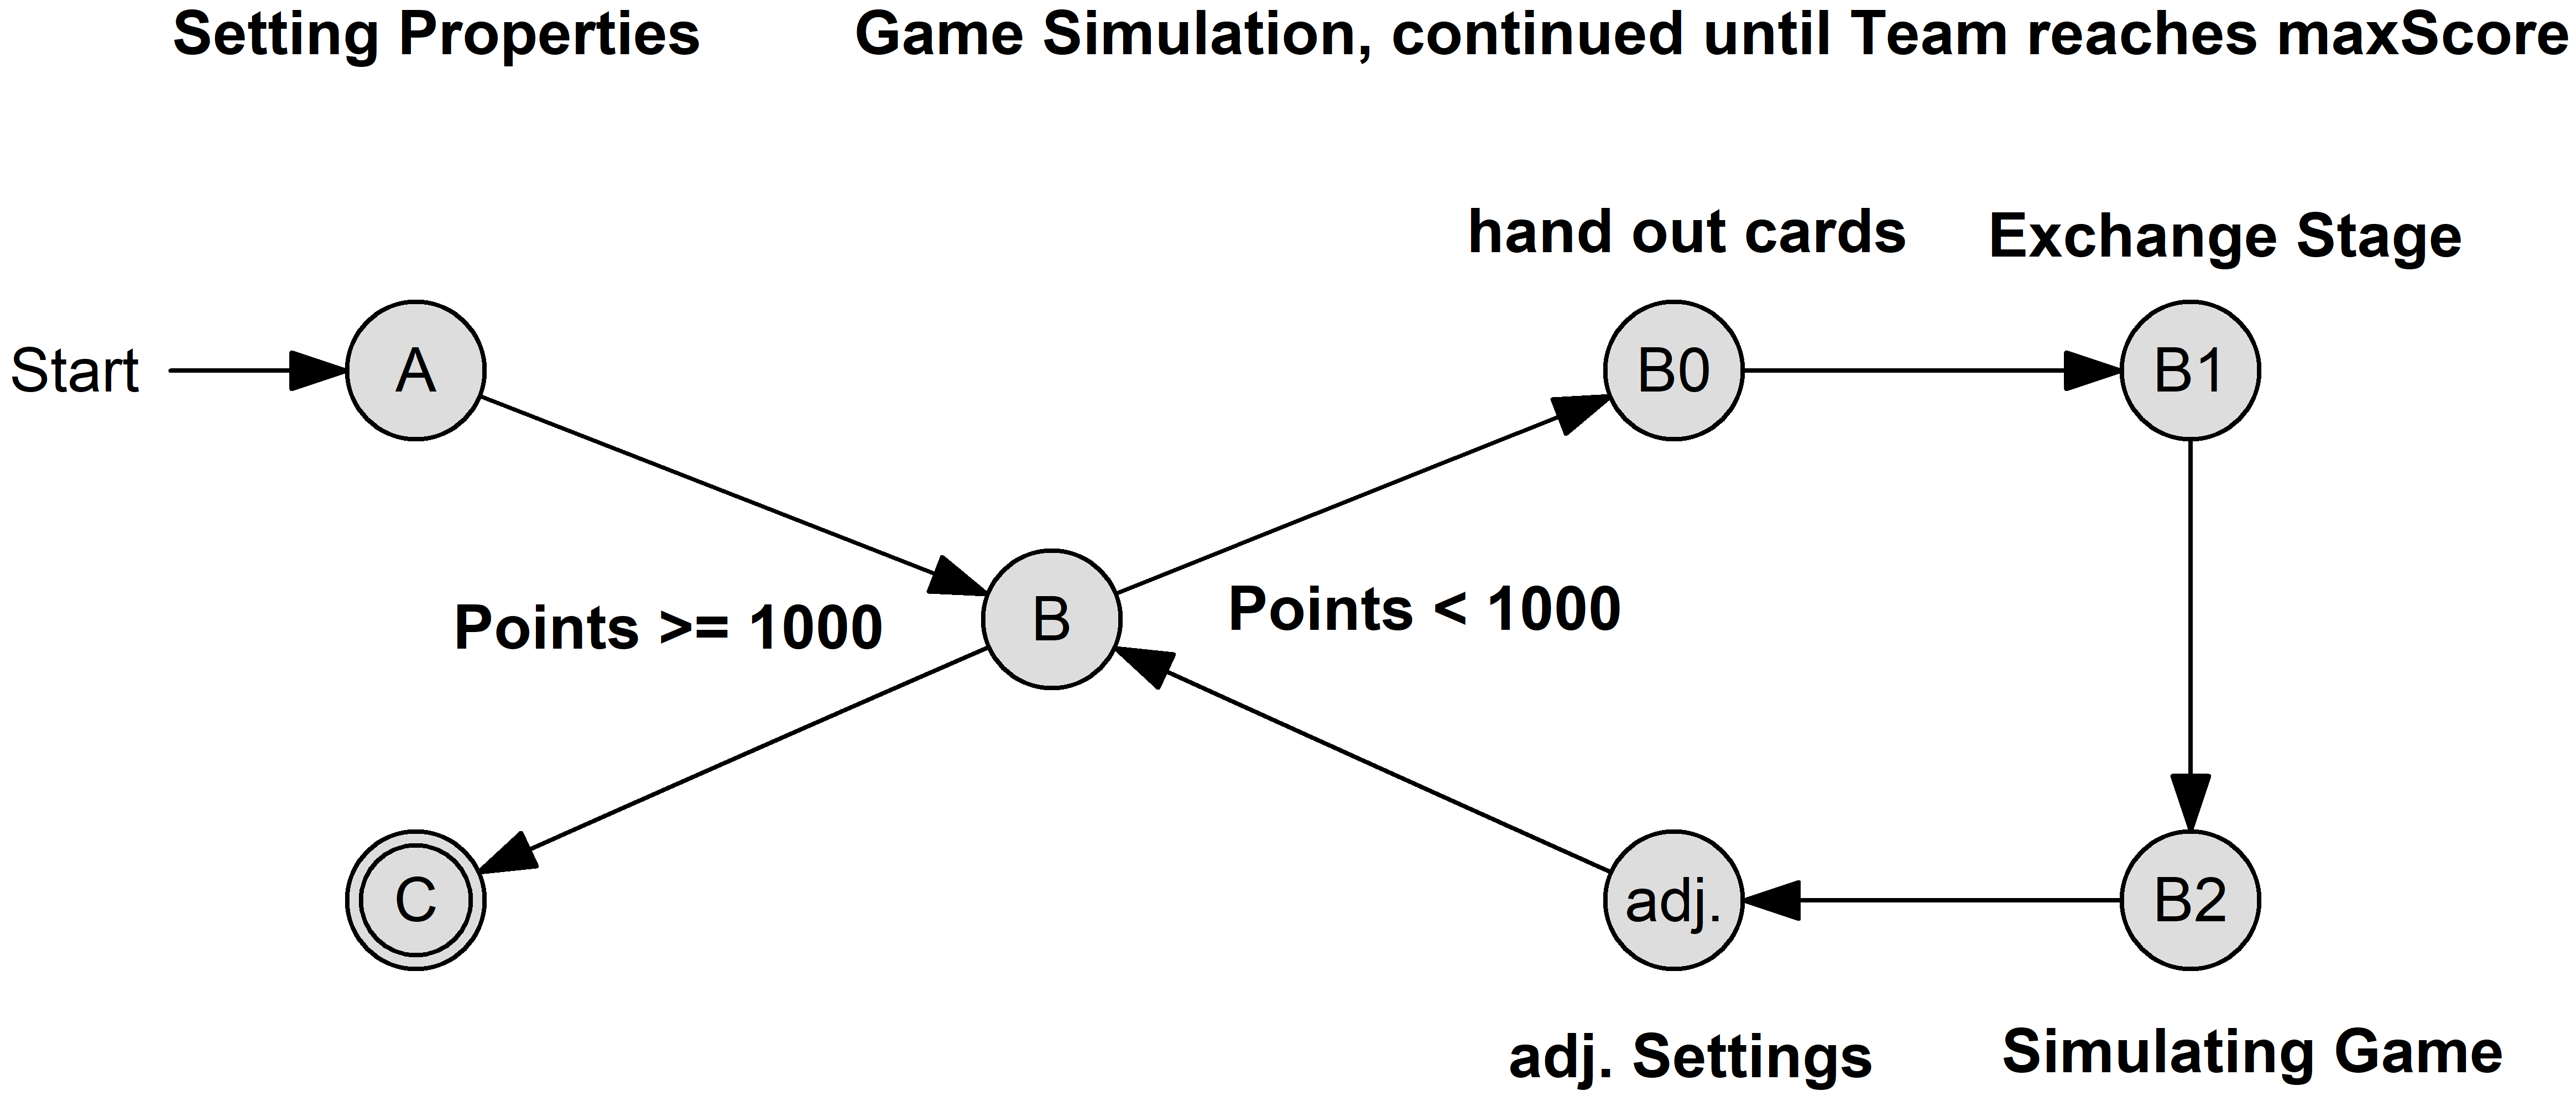
\includegraphics[width=0.5\textwidth]{Bilder/graph}
    \caption{Game model}
    \label{fig:meine-grafik}
\end{figure}

The game up to 1000 points is represented as a game tree.
At the beginning 4 players, divided into 2 teams enter the game (A). We will set $\alpha$ and $\beta$. 
The next part of the game (B) will be repeated until the score reaches at least 1000 points. We divided it into three subgames (B.0, B.1, B.2).
First, we will give every player a set of cards (B.0). This set of cards will be represented by a value $X_i$ in [0,1]. The sum of all sets can be higher than 1 in total. The value of the set is not connected to single cards but to a probability to play these cards in combinations. We will discuss this in detail later on.

In the basic model, B.0 is only connected to statistics and no game in meanings of game theory. Later on, we can introduce game-theoretical elements to this subgame. 

The second part (B.1) represents the “Exchange Stage”. Depending on his Cards and his strategy, every player will give away three $\Delta x$ and will receive three $\Delta x$ which can be positive or negative. The payoff will be represented by a Util$\in [0,1]$ with "new" card values.

The third subgame (B.2) takes the card values X from subgame B.1 and the score. They are used to determine the outcome of the actual game, reflecting on the players strategies and possibilities to take a higher risk because of the score. This will result in a Util function which allocates the 100 points (and additional Tichu-points) to the teams. 

To every game B, the parameters $\alpha, \beta, \gamma, \delta$ are considered and can be adjusted.  
The repetition of subgame B will end when one team reaches at least 1000 points. 

In first approximations we will also consider $\beta$ and $\gamma$ as invariant. 

\subsubsection{Subgame A}
To start a round of Tichu, we will assign a player $\alpha_i$ and $\beta_i$. As assumed before, all $\beta_i$ are equal. Therefore, we will have two options on $\beta$ and 16 options on $\alpha$. Some of those options are only permutations, because of the team-aspect. We will reduce the number of possible $\alpha$ to 6 as shown in the table. We will call this combination $\tilde{\alpha}_i$: \\
\begin{table}[h]
\resizebox{0.5\textwidth}{!}{%
\begin{tabular}{|c|c|c|}
\hline 
Player 1 $\backslash$ Player 2 & A & B \\ 
\hline 
A & 1 (AA) & 2 (AD = DA) \\ 
\hline 
B & 2 (DA = AD) & 3 (DD) \\
\hline 
\end{tabular}%
}
\end{table}
\begin{table}[h]
\resizebox{0.5\textwidth}{!}{%
\begin{tabular}{|c|l|l|l|}
\hline 
Player 1 $\backslash$ Player 2 & 1 & 2 & 3 \\ 
\hline 
1 & $\alpha_1$ (AAAA) & $\alpha_2$ (AAAD) & $\alpha_3$ (AADD) \\ 
\hline 
2 & $\alpha_2$ (ADAA) & $\alpha_4$ (ADAD) & $\alpha_5$ (DDAD) \\ 
\hline 
3 & $\alpha_3$ (DDAA) & $\alpha_5$ (ADDD) & $\alpha_6$ (DDDD) \\ 
\hline 
\end{tabular}%
} 
\end{table}
\subsection{Subgame B.0}
In our basic model, B.0 is invariant under all $\alpha$, $\beta$, $\gamma$ and $\delta$. It is only based on statistics. 
To start off with a simple approximation, we assign $X_i$ to be an element of the normal distribution with parameters $\mu$, $\sigma$.
Our first assumptions is, that we set $\mu$ to 0.5 and will define $X_i$ higher or equal to 1 as 1,  $X_i$ lower or equal to 0 as 0.   
According to this definition, $X_i$ is always in $[0,1]$. We will set $\sigma$ later according to realistic data and surveys. We will now assume that we will always get an $X = \{X_1, …, X_4\}$ from subgame B.0. This will be the card value used in later games. 

\subsection{Subgame B.1}
To understand the “Exchange Stage”, we have to give some basic information on Tichu which leads to our approximation of this subgame. First of all we definie some terms:
\begin{definition}["good" cards]
"Good" cards are for example bombs, high cards like ace or long, specific combinations that other players do not have.
\end{definition}
\begin{definition}["bad" cards]
Bad cards can rarely be played, for example deep cards or combinations that are never the highest combinations, so you rarely win a trick
\end{definition}
\begin{enumerate}
\item A player can give “good” cards to his partner if and only if he has “good” cards.
\item A player can give “bad” cards to his opponents if and only if he has “bad” cards. 
\item The value of a card is subjective to a player. 
\item There is no absolute solution for every situation, the best solution is subjective to a player \\
\end{enumerate}
\begin{definition}[Player, Team, Partner and Opponent]
Given $\alpha$, $\beta$ and $X$, a player $P_i$ is called the triple ($\alpha_i$, $\beta_i$, $X_i$). 
On the set of players, we define an equivalence relation, where each class forms a Team $T_j$. Following conditions are true for players A ($\alpha_A$, $\beta_A$, $X_A$), B($\alpha_B$, $\beta_B$, $X_B$), C($\alpha_C$, $\beta_C$, $X_C$):
 \begin{axioms}[(P1)]
  \item A $\sim $ B (Reflexiv)
  \item A $\sim$ B $\Leftrightarrow$ B $\sim$ A (Symmetric)
  \item A $\sim$ B, B $\sim$ C $\Rightarrow$ A $\sim$ C (Transitivity)
  \end{axioms}
Players in the same Team will be called partners while players in another Team will be called opponents. We will write $PT_i$ for the Partner Team of $P_i$ and $OT_i$  for the Opponent Team of $P_i$.

We define $T_1 = [P_1,P_2]$  and $T_2 = [P_3,P_4]$. Therefore, $PT_1 = T_1$, $OT_1 = T_2$, $PT_2 = T_2$, $OT_2 = T_1$.

\end{definition}

\begin{definition}[Symmetric game perspective]
We will say, two players $P_i$, $P_j$ with  $i \neq j$ share a symmetric game perspective if $P_i = P_j$, $PT_i = PT_j$, $OT_i = OT_j$, in words: They have the same cards and the teams are identically from their point of view. 
\end{definition}
\begin{definition}[Total Exchange-Function]
We assume we have given $\alpha$, $\beta$, X. A function $\pi: \{0,1\}^8 \times [0,1]^4 \to [0,1]^4, (\alpha, \beta, X) \mapsto (X’)$ will be called an Exchange-function to B.1  if it applies to the following rules:
\paragraph{Randomness and Average}
$\alpha$, $\beta$, X are fixed. Then there is $\Delta X \subset [0,1]^4$ with $X’ \in \Delta X$. We will write $\pi^* (\alpha, \beta, X) = X^* \in \Delta X$ for the average of $\pi(\alpha, \beta, X)$. $\pi^*$ is a well-defined function, while $\pi$ allows random values around $\pi^*$.
\paragraph{Continuous and monotony of X}
$\alpha$, $\beta$ and X are fixed. If we change X in only one value that $X_i$ becomes $wide\hat{X_i}$, it applies to the following rules:
\begin{axioms}[(C1)]
\item $\forall \epsilon > 0, \exists \delta > 0$ with $| X_i - \widehat{X_i}| < \delta$ \\$\Rightarrow | \pi^*(X_i) - \pi^*(\widehat{X_i}) | < \epsilon $
\item $\widehat{X_i} \leq X_i \Rightarrow \pi^*(\widehat{X_i}) \leq \pi(X_i)$
\end{axioms}

\paragraph{Symmetric outcome}
If two players $P_i$, $P_j$ have a symmetric game perspective, $\pi^*(X_i) = \pi^*(X_j)$
\end{definition}

Based on our approximations of the subgame, we now try to construct an Exchange Function. First of all, we try to create an easier function, which describes how a single Player selects cards he wants to give away. If we only look at this function, we will see some facts:

\begin{axioms}[(F1)]
\item For Player $P_i$, only $\alpha$, $\beta_i$ and $X_i$ are relevant.
\item Player $P_i$ does not differ between Opponents. 
\item The Player $P_i’s$ strategy does not change his behaviour on Opponents. 
\item In fact, he only needs to know his strategy, who he selects cards for and if known, his partner’s strategy. 
\end{axioms}

We put these facts together in a Diagram (the numbers represent diffrent exchange functions and $P_P$ - is a Player passing; $P_R$ - is a Player receiving):

\begin{table}[h]
\caption{Table 1.1} \bigskip
\label{tab:my-table}
\resizebox{0.5\textwidth}{!}{%
\begin{tabular}{l|l|ll|l|ll|}
\cline{2-7}
                                          & \multicolumn{3}{l|}{$\beta_i = 0$} & \multicolumn{3}{l|}{$\beta_i=1$} \\ \hline
\multicolumn{1}{|l|}{\multirow{3}{*}{OT}} & $P_R \backslash P_P$           & A         & D         &           & A         & D        \\ \cline{2-7} 
\multicolumn{1}{|l|}{}                    & A          & 1         & 1         & A         & 2         & 2        \\
\multicolumn{1}{|l|}{}                    & D          & 1         & 1         & D         & 2         & 2        \\ \hline
\multicolumn{1}{|l|}{\multirow{3}{*}{PT}} & $P_R \backslash P_P$              & A         & D         &           & A         & D        \\ \cline{2-7} 
\multicolumn{1}{|l|}{}                    & A          & 3         & 4         & A         & 5         & 6        \\
\multicolumn{1}{|l|}{}                    & D          & 3         & 4         & D         & 7         & 8        \\ \hline
\end{tabular}%
}
\end{table}
\paragraph{1.}
The Player is exchanging with an unknown Opponent. Therefore he will select a “bad” card, independent of his own strategy
\paragraph{2.}
The Player knows his opponent. He will also give him a “bad” card. The only difference is, that he knows better how the player will react on the card. This will change how an Opponent receives the card, but is equivalent to 1. 
\paragraph{3./4.}
The Player gives cards to his Partner depending on his strategy. He does not know the strategy of his Partner.
\paragraph{5.-8.}
The Player knows his own and his Partners strategy. Therefore his results will be better and the card difference will change. 

\begin{definition}[Pass-Function]
A function $\xi_{ji} : \{0,1\}^5 \to [-1,1], (\alpha, \beta_i) \to \hat{\xi}_{ji}$ will be called a pass function, if it describes what $P_i$ gives to $P_j$ according to certain rules:
\paragraph{Randomness and Average}
$\alpha$, $\beta_i$ are fixed. Then there is $\Delta  \hat{\xi_{ji}} \subset [-1,1]$ with  $\hat{\xi_{ji}} \in \Delta  \hat{\xi_{ji}}$. We will write $\{xi_{ji}\}^* (\alpha, \beta_i) =  \hat{\xi_{ji}} \in \Delta  \hat{\xi_{ji}}$ for the average of $\xi(\alpha, \beta_i)$. $\xi_{ji}^*$ is a well-defined function, while $\xi$ allows random values around $\xi^*$.
\paragraph{Symmetric outcome}
If two players $P_i$, $P_j$ have a symmetric game perspective towards each other,  $\hat{\xi_{ji}}^* =  \hat{\xi_{ji}}^*$
\paragraph{Normative aspects}
$\sum_{j = 1}^4 \hat{\xi_{ji}} = 1$
\paragraph{Realistic passing}
$\hat{\xi_{ii}} >>  \hat{\xi_{ji}}$ with $ i \neq j $
\end{definition}
\begin{definition}[Receive-Function]
A function $\eta_{ji}: \{0,1\} \times [-1,1] \to [-1,1], (\beta_i,  \hat{\xi_{ji}}) \mapsto \hat{\eta_{ji}}$ will be
called a “Receive-Function”, if it describes how $P_j$ receives cards from $P_i$ according to certain rules:
\paragraph{Randomness and Average}
$\beta_i$, $\hat{\xi_{ji}}$ are fixed. Then there is $\Delta  \hat{\eta_{ji}} \subset [-1,1]$ with  $\hat{\eta_{ji}} \in \Delta  \hat{\eta_{ji}}$. We will write $\{\eta_{ji}\}^* (\beta_i, \hat{\xi_{ji}}) =  \hat{\eta_{ji}} \in \Delta  \hat{\eta_{ji}}$ for the average of $\eta(\beta_i, \hat{\xi_{ji}})$. $\eta_{ji}^*$ is a well-defined function, while $\eta$ allows random values around $\eta^*$.
\paragraph{Symmetric outcome}
If two players $P_i$, $P_j$ have a symmetric game perspective towards each other:  $\hat{\xi_{ji}}^* =  \hat{\xi_{ij}}^*$
\paragraph{Self passing}
$\eta_{ii}(\hat{\xi_{ii}}) = \hat{\xi_{ii}} $
\end{definition}
\begin{definition}[Exchange-Function]
A function $\lambda_{ji}: \{0,1\}^5 \to [-1,1], \lambda_{ji} = \eta_{ji} \circ \xi_{ji}$ with $\eta_{ji}$ a Receive-Function and $\xi_{ji}$ a Pass-Function with existing $\alpha$, $\beta_i$.
\end{definition}
\begin{remark}[Construction]
We will now construct a Total Exchange Function based on an Exchange Function $\lambda_{ji}$. We will define $\Lambda = (\lambda_{ji})$ as a quadratic matrix. 
The Total Exchange-Function will be $\Lambda: X \mapsto \Lambda X = X’$
We now have to prove that this construction fits the definition.
\begin{axioms}[(1)]
\item Randomness and Average: This is induced from the combination of $\xi_{ji}$ and $\eta_{ji}$ in every argument. Therefore we can find an $\Delta \Lambda$ and $\Lambda^* $ which lead to $\Delta X $ and 
$X^*$
\item $\Lambda^*$ is a linear function, therefore continuous and monotone
\item Symmetric outcome is induced from the combination of $\xi_{ji}$ and $\eta_{ji}$ in every argument as in 1
\end{axioms}
We have now created a matrix $\Lambda$ which describes the Exchange Stage. To complete the definitions, we will introduce $ \Pi : \{0,1\}^8 \to M(4 \times 4, \mathbb{R}), (\alpha, \beta) \mapsto \Lambda $
\end{remark}

\subsection{Subgame B.2}
We shall now explore the active game, i.e. the laying and trumping of cards. We will first define a few new terms and three basic functions, including a double win probability function as well as a tichu announcement and tichu win probability function. We will then simulate the theory of an entire game consisting of multiple rounds and establish the different possible cases that can occur throughout a round.

We further assume players are completely rational and do not harm their own chances. Concretely, we presuppose that no counter-tichu will be called on a teammate’s tichu announcement. At this stage we can therefore treat two teammates as simply one element.

As a reminder, teams are defined by combining the two player triples $P_1$, $P_2$ and $P_3$, $P_4$into one element $T_1 = \{P1,P2\}$ and $T_2 = \{P3,P4\}$.

We shall start by defining the relevant terms and functions needed for this discussion. Let S define the game score, given by $S = \{S_1, S_2\} \in \mathbb{Z}^2$ where $S_1$ and $S_2$ are the scores of $T_1$ and $T_2$ respectively.

\begin{definition}[Double Win Function]
For each team we define a double win function $D_i(T_1, T_2)$.
\begin{align*}
D_i: ({0,1}^5 \times [0,1])^4 \to [0,1] (T1,T2) \mapsto d_i
\end{align*}
\end{definition}
This function returns the probability of a double win of each team for a round. As teams are always aiming for this bonus through a double win, we describe this function as independent of the current score and probably more dependent on the team strategies and the value of the cards. Whether or not player strategies have any influence on this probability will be heuristically/ empirically determined in the realisation section of this essay.

Next, as scoring a Tichu requires both calling and winning a Tichu, we separate the Tichu scoring opportunity into a Tichu announcement and Tichu winning function. For each team we define a Tichu announcement function $C_i(T_i, S)$, where $T_i$ are the respective teams and S is the current score. 


\begin{definition}[Tichu Announcment Function]
For each team we define a Tichu announcement function $C_i(T_i, S)$, where $T_i$ are the respective teams and S is the current score:
\begin{align*}
C_i: ({0,1}^5 \times [0,1])^2 \times \Z^2 \to [0,1] (T_i,S) \mapsto c_i
\end{align*}
\end{definition}
This function returns the Tichu announcement probability of each team for a round. It depends on a host of different variables including the player and team strategies as well as the current score and score difference. Such a function allows us to, for example, represent a greater probability of calling a Tichu when the opposing team has a large score margin or is very close to 1000 points.


\begin{definition}[Tichu Win Function]
Finally, we define the Tichu winning function $W_i(X_1, X_2,X_3,X_4)$ for each team as follows.
\begin{align*}
W_i: [0,1]^4 &\to [0,1] \\(X_1,X_2,X_3,X_4) &\mapsto t_i
\end{align*}
\end{definition}
This function indicates the probability that a team wins their Tichu bet in a given round. This too, is independent of score and game strategies as both teams will always want to win the Tichu bet. Rather, it depends completely on the teams’ card values.

With the above functions we can now simulate the theory of an entire game consisting of multiple rounds and establish the different possible cases that can occur throughout a round. We shall first explain how we simulate the probability of one or multiple Tichu calls and the scoring of a double win. Next, we shall explain how we calculate points for a team and then explore the following possible scenarios case by case.

\begin{definition}[binary random varibale]

We initially want to define a helper function, namely a \textbf{binary random variable} $Z(x): [0,1] \to [0,1]$ as a random variable that takes the value 1 with probability $x$ and $0$ with probability $1-x$.

\end{definition}

\subsubsection{Course of the game}
At the beginning we determine, through two binary random variables $Z(c_1)$ and $Z(c_2)$, whether team 1 or 2 announces a Tichu $(Z(c_1) = 1$ or $Z(c_2) = 1)$. Similarly, a binary random variable $Z(d_1)$ determines whether team 1 makes a double victory $(Z(d_1) = 1)$ or not $(Z(d_1) = 0)$. If $Z(d_1) = 0$, another binary random variable $Z(d'_2)$ determines if team 2 makes a double victory $(Z(d'_2) = 1)$ or not $(Z(d'_2) = 0)$. $d'_2$ is given by $d'_2 =d_2\cdot\frac{1}{1-d_1}$ because this case is only determined in $1-d_1\cdot 100$ percent of the cases. If $Z(d_1) = 1$, then $Z(d_2)$ is automatically 0, since a double victory of one team strictly excludes a double victory of the other.

Here we make the first differentiation between cases depending on whether a double win is scored or not. This is because a double win immediately awards +200 points to the scoring team regardless of the points distribution during the round. If a double win is not achieved by either team the points distribution must be calculated.

In the case $Z(d_1) = 1 \lor Z(d_2) = 1$, i.e. a double victory has been achieved, the score of team $T_i$ for which $Z(d_i) = 1$ applies will be increased by 200 points $(S_i += 200)$. Furthermore, if $Z(c_i) = 1$, Team $T_i$ has won its announced Tichu and therefore gets another 100 points $(S_i += 100)$. However, if the opposing team $T_j (i != j)$ has announced Tichu $(Z(c_j) = 1)$, this team loses 100 points $(S_j -= 100)$ as the calling player was unable to exit the round first.

The alternative case, $Z(d_1) = 0 \land Z(d_2) = 0$, requires more theory as we must determine how many points each team scores during a round. We assume that the announcement of Tichus has no effect on the distribution of points, although the opposing team may, for example, prioritise exiting the round first over scoring maximum points through won card values. We argue any such shift by a Tichu announcement in any specific round would generally be balanced out over all rounds of the game. Thus, we must only determine the points scored through the distribution of won cards.

For this calculation, we introduce two normally distributed random variables $n_1$ and $n_2$ whose mean value and standard deviation are to be determined in the realisation section of this essay. The purpose of these random variables is to simulate the fluctuations in scores obtained every round by both teams throughout the game. This will be explained further in the next section. The scored points for a round are to be calculated as follows: Let $X_{tot} = \sum_{i=1}^{4} X_i$ be the total sum of card values in this round, then
\begin{align*}
    &\Delta S_1 = (X_1\cdot n_1 + X_2\cdot n_2)/ X_{tot} \cdot 125 - 25\\
    &\Delta S_2 = (X_3\cdot n_1 + X_4\cdot n_2)/ X_{tot} * 125 - 25\\
\end{align*}
represent the change in score for each team for a round, where $\Delta S_1$ and $\Delta S_2$ are rounded to the nearest multiple of 5. Thus the change in score is calculated as a percentage of the card values for a specific round. The correctional factors 125 and -25 as well as the rounding serve to adjust the point value to the frame of a Tichu round.

Compounded onto the above theory are the following three cases as they relate to possible Tichu scenarios, namely: none, one or both teams announcing a Tichu:

\begin{axioms}[(C1)]
\item   If no team announces a Tichu $(Z(c_1) = 0 \land Z(c_2) = 0)$, then the point changes are simply added to the score.
\begin{gather*}
S_1 += \Delta S_1 \qquad S_2 += \Delta S_2
\end{gather*}
\item If one of the teams announces a Tichu $(Z(c_1) = 1$ XOR $Z(c_2) = 1)$ then a binary random variable $Z(w_i)$ determines whether this team makes the announced tichu. Here $w_i$ is, as defined earlier, the team's win probability. If $Z(w_i) = 1$ then the change of points is
\begin{gather*}
S_i += \Delta S_i + 100 \qquad S_j += \Delta S_j
\end{gather*}
Where $S_j$ represents the score of the opposing team. If $Z(w_i) = 0$ for the announced Tichu, then 100 points are subtracted from $S_i$. Other than that, the scores are added up as in case 1.
\item Both teams have announced a Tichu $(Z(c_1) = 1 \land Z(c_2) = 1)$. Since we assume every player to be rational, we assume that one of the two Tichus is definitely made. Now the probability that team 1 will make the Tichu is $w'_1 = \frac{w_1}{w_1+w_2}$, while $w'_2 =\frac{w_2}{w_1+w_2} = 1- w'_1$ represents the probability for team 2. Again, with the help of a binary random variable $Z(w'_1)$, we determine whether team 1 $(Z(w'_1) = 1)$ or team 2 $(Z(w'_1) = 0)$ has made the Tichu. If $T_i$ makes the Tichu and $T_j$ is the opponent team, the score is:

\begin{gather*}
S_i += \Delta S_i + 100 \qquad S_j += \Delta S_j - 100
\end{gather*}
This completes a round of the game. Now the subgames $B.0,B.1,B.2$ are repeated until $S_1 > 1000$ or $S_2 > 1000$ applies. In the following flowchart the process of $B.2$ is visualized once again:
\end{axioms}
(Schaubild)
\section{Realisation}
We will now adjust our basic model to realistic data which helps to achieve an approximation of Tichu. We will not change $\alpha$ and $\beta$ during the game. Therefore we will start with modeling a function for B.0.

\subsection{Subgame B.0}
In our basic approach, we assume an average hand to have a value $X_i$ = 0.5, this value is based on the data from tichuonline.ch, the winning rate is almost normal distributed by 0.5 with (skewness) to 0, in our idealistic scenario we assume that the distribution is symmetric. $X_i$ = 0 has no chance in winning the game and $X_i$ = 1 is equal to an guaranteed win. The only question is, to which percentage do we get really good cards? Assuming, the card value is symmetric around 0.5, we can agree, that instant loose and guaranteed win are very rare. We now have to make an arbitrary choice, which value corresponds to which card combinations. 
Given, that a Great Tichu is only won in 2.21$\%$ of all games, We will set $P(X_i \geq 0.9) = 0.221$, the share of Winning a great Tichu in reference to all games. This gives us a $\sigma$ of 0.199. A Tichu is only won in 8.53$\%$ of all games, which is equal to $X \geq 0.78$
We will receive this plot which shows the possibility to get cards with a certain value.
\begin{figure}[h]
    \centering
    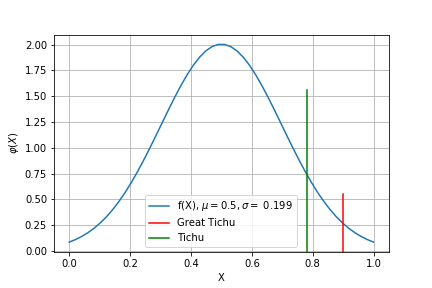
\includegraphics[width=0.5\textwidth]{Bilder/cards_distribution}
    \caption{cards distribution}
    \label{fig:meine-grafik}
    \centering
    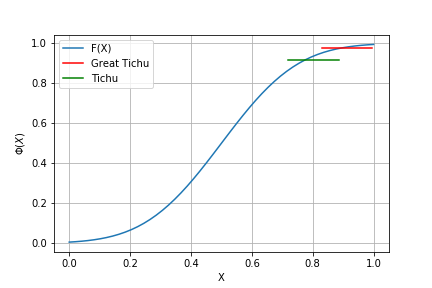
\includegraphics[width=0.5\textwidth]{Bilder/cards_distribution_cumultative}
    \caption{cards distribution cumultative}
    \label{fig:meine-grafik}
\end{figure}
\\ \\We will always use this approximation and will not discuss it furthermore.
\subsection{Subgame B.1}
To approximate the game, we will start with the most simple approach possible. A player can only pass one card, he has 14 cards on his hand. Therefore, if he passes all cards away, the average value will be $\frac{X}{14}$. This is not a perfect approximation, but it will work for the beginning. Later on, we can redefine this value if necessary. 

Keeping it easy, we will start looking at the exchange with an enemy. We only discovered one difference, whether the Player knows his Opponents strategy or not. But this difference is marginal and we will do not distinguish between these cases in this approach. 
Therefore, there is only one possible function towards an Opponent. We will call this function $\xi_O$ and assume it as normal distributed. We will set $\mu = 0$, because normally giving away one card does not change the value of your hand. According to our “stupid approach”, we will set $2\sigma = \frac{1}{14}$, because it is the value of an average card in most of the cases (further explanation in work). \\
\begin{figure}[h]
    \centering
    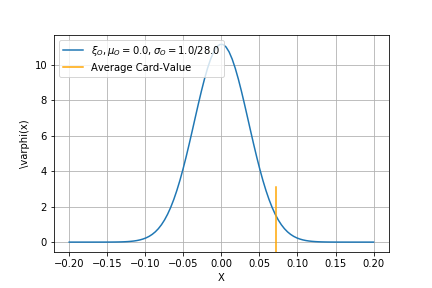
\includegraphics[width=0.5\textwidth]{Bilder/pass_function_ot}
    \caption{pass function for oppoenent player}
    \label{fig:meine-grafik}
    \centering
    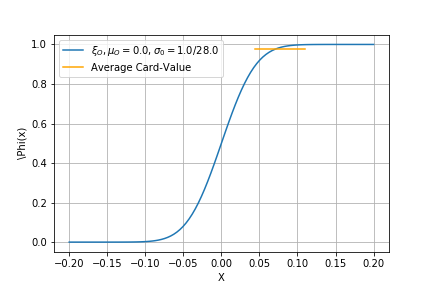
\includegraphics[width=0.5\textwidth]{Bilder/pass_function_ot_cumultative}
    \caption{pass function for the opponent player cumultative}
    \label{fig:meine-grafik}
\end{figure}
\\
The Pass-function towards your partner is more difficult to define: To realize it, let us imagine you are a new player to this game. You have no strategy and no knowledge. So every card is equal to you and as described before, the average card value is $\frac{X}{14}$. The cards are probably normal distributed within a wide range. Therefore we define $\xi_P$ as the Pass Function towards a Partner with $\mu_P = \frac{1}{14}$ and $\sigma_P = \frac{1}{14}$. 

If a player is aggressive, he will pass cards with less value and if he is defensive, he will pass cards with higher value. If he knows, his partner is defensive, he will pass lower cards and if he knows, that his partner is aggressive, he passes higher cards. This leads us to the following table:  \\
\begin{table}[h]
\caption{Table 2} \bigskip
\label{tab:my-table}
\resizebox{0.5\textwidth}{!}{%
\begin{tabular}{|l|ll|l|ll|}
\hline
\multicolumn{3}{|l|}{$\beta = 0$} & \multicolumn{3}{l|}{$\beta=1$} \\ \hline
\textit{$P_R \backslash P_P$}      & A       & D      & $P_R \backslash P_P$         & A        & D        \\ \hline
A              & -1      & +1     & A        & 0        & +2       \\
D              & -1      & +1     & D        & -2       & 0        \\ \hline
\end{tabular}%
}
\end{table}
We can construct a formula using this table: 
\begin{equation*}
z_{ji} = (1 - 2\cdot\alpha_i) + \beta_i \cdot (2\cdot\alpha_j - 1)
\end{equation*}
We will set $\mu = \mu_P + \frac{\sigma_P}{2} \cdot z_{ji}(\alpha, \beta)$. This will give us one function for $\xi_P$:
\begin{figure}[h]
    \centering
    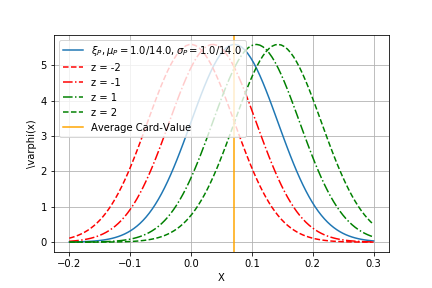
\includegraphics[width=0.5\textwidth]{Bilder/pass_function_p}
    \caption{pass function for your team partner}
    \label{fig:meine-grafik}
    \centering
    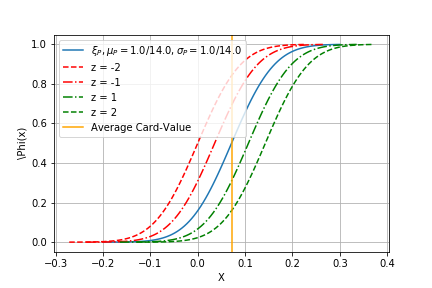
\includegraphics[width=0.5\textwidth]{Bilder/pass_function_p_cumultative}
    \caption{pass function for your teampartner cumultative}
    \label{fig:meine-grafik}
\end{figure}
\\
A card which has a negative value to player $P_i$ can have a positive value to $P_j$ (can complete a bomb). Therefore the value can change during the exchange from $\hat{\xi}_{ij}$ to $\hat{\eta}_{ij}$. In this approach, we will set $\eta_{ij} = id$, because the effect is very small in a large number of games. 

We now have created Pass-functions $\xi_{ji}$ and a Receive-Function $\eta_{ji} = 1$. We can use this functions to analyse the outcome of the Exchange-Stage $\lambda_{ji} = \xi_{ji}$. We can write $\Lambda$ using the average:
\begin{gather*}
\Lambda = \begin{pmatrix} 
1 - \xi_{21} & \xi_{12} & 0 & 0 \\
\xi_{21} & 1 - \xi_{12} & 0 & 0 \\
0 & 0 & 1 -  \xi_{43} & \xi_{34} \\
0 & 0 &  \xi_{43} & 1 - \xi_{34} \\
\end{pmatrix}
\end{gather*}

\subsection{Subgame B.2}
With the actual Tichus play there are several combinations and possibilities how this can run off. Especially decisive can be for example, who starts. Because of the combination of the cards it could be that all 4 players have the possibility to announce the Tichu. To approximate this problem as best as possible, we have considered that we simply look at the probability of winning Tichu, rather than the individual hand cards.

So first we will calculate the probability that a certain team will announce a Tichu. However, this will be done independently of the cards, because we assume that we simulate so many games that the average probabilities of winning the tichu fit better than imaginary probabilities of each card.
We assume that the team announces a tichu and not the single player. There are in theory game situations in which both team partners announce a tichu, but since we assume common knowledge, these situations are extremely rare. For example, player 1 from team 1 and player 2 from team 2 has announced a tichu. Player 3 from team 1 notices that player 1 probably won't make it and says tichu himself and wins it. This case occurs very rarely, because it requires, among other things, that player 3 has not yet played a card and is already sure that he will make the tichu and his partner will not.
In addition, we say that if both teams announce, one of the two teams will surely win the Tichu. Of course, in theory a third player could win the game (even without announcing Tichu), but this player would also have to be sure that his partner will not make it, because otherwise the common knowledge would be violated. But since this situation of absolute certainty about the cards of the partner is very rare, we neglect this case here.

So to calculate the probabilities for the announcement of the Tichu, we need 2 basic factors:
\begin{enumerate}
\item Basic aggressiveness of the players (team$_{\alpha_1}$,team$_{\alpha_2}$)
\item  Additional risk tolerance depending on the score
\end{enumerate}
The basic aggressiveness of the players is converted to a basic aggressiveness of the team. This basic aggressiveness is derived from the player model.
The willingness to take risks increases. However, this cannot be directly dependent on the player model, because due to the common knowledge, both the defensive and the aggressive player must be prepared to take extreme risks at some point.
To determine this, we have conducted a survey. It asks for the willingness to take risks in 3 categories:
\begin{enumerate}[(1)]
\item diffrence in scores
\item edge of wedge
\item own distance to victory
\end{enumerate}
The scale here was the willingness to take risks from 1 to 10, whereby in category (1) and (2) 10 meant a lot of risk and 1 normal. For (3), 1 was normal risk and 10 was particularly low risk.
 As the survey revealed, Category (1) > Category (2) > Category (3) is in the ranking. The fluctuations in category (1) are 5 points.
 For category (2) 2.5 points and in (3) 0.5 points. In this weighting, these categories are also considered in the function.
The survey revealed the following data points (based on this point we generated with numpy a regression):
\paragraph{Cat.1}
$X=[0,100,200,300,400,500,600,700,800,900]$ \\ \\
$Y=[\frac{86}{21},\frac{83}{21},\frac{96}{21},\frac{114}{21},\frac{122}{21},\frac{142}{21},\frac{150}{21},\frac{170}{21},\frac{180}{21},\frac{183}{21}]$\\
\paragraph{Cat.2}\par
$X=[100,200,300,400,500,600,700,800]$ \\ \\
$Y=[\frac{140}{21},\frac{133}{21},\frac{111}{21},\frac{105}{21},\frac{100}{21},\frac{89}{21},\frac{88}{21},\frac{93}{21}]$\\
\paragraph{Cat.3}\par
$X=[100,200,300,400,500,600,700,800]$\\ \\
$Y=[\frac{94}{21},\frac{104}{21},\frac{105}{21},\frac{92}{21},\frac{105}{21},\frac{104}{21},\frac{92}{21},\frac{94}{21}]$
\begin{figure}[h]
    \centering
    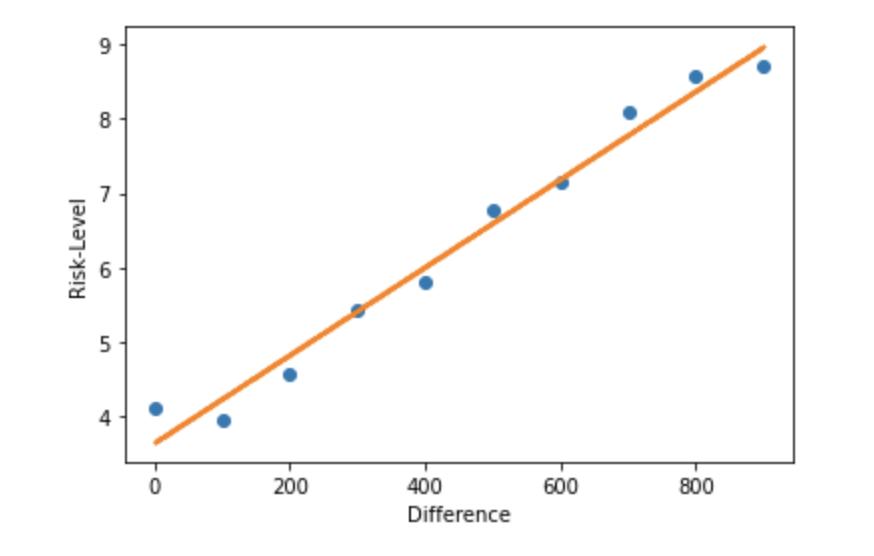
\includegraphics[width=0.5\textwidth]{Bilder/risk_level_diffrence_200steps}
    \caption{$f_1(x)=0.00591631\cdot x+3.65194805$}
    \label{fig:meine-grafik}
\end{figure}
\begin{figure}[h]
    \centering
    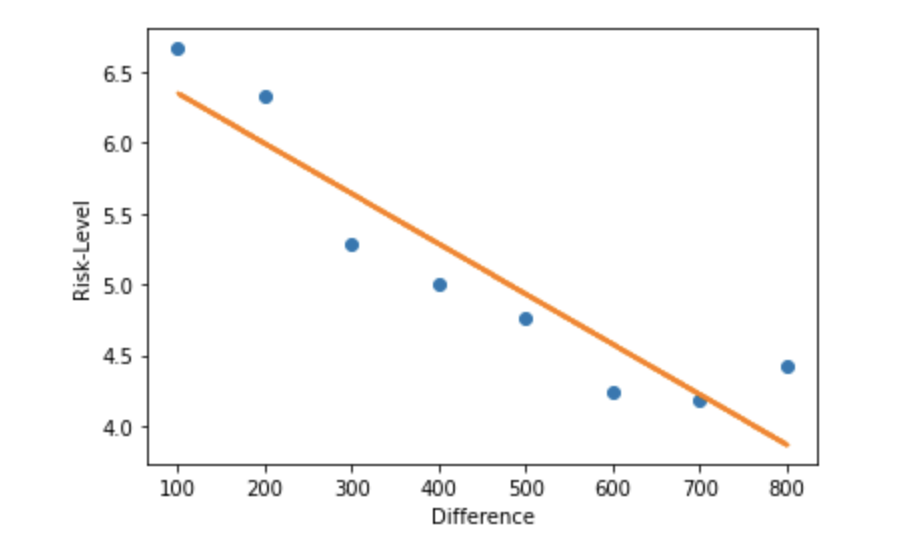
\includegraphics[width=0.5\textwidth]{Bilder/risk_level_diffrence_100steps}
    \caption{$f_2(x)=-0.00354308390\cdot x+6.70748299$}
    \label{fig:meine-grafik}
\end{figure}
\begin{figure}[h]
    \centering
    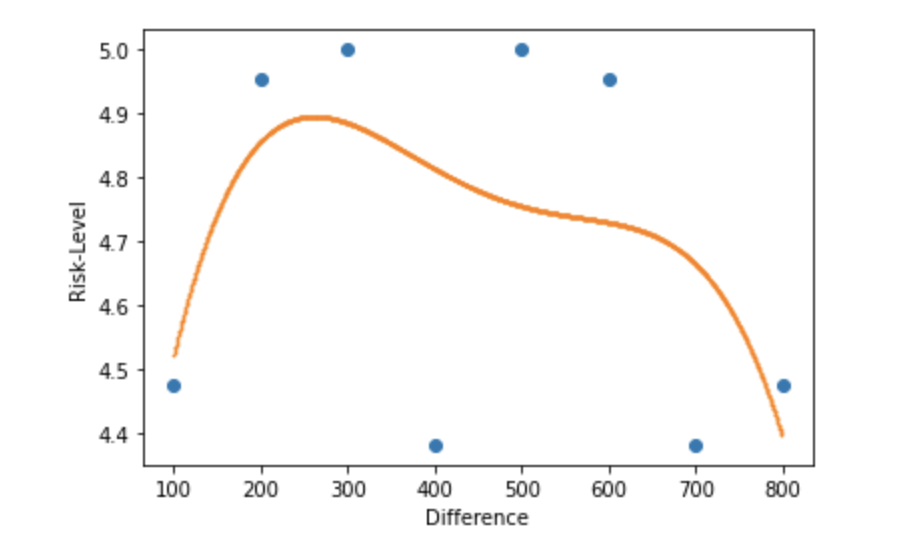
\includegraphics[width=0.5\textwidth]{Bilder/risk_level_diffrence_nonlinear}
    \caption{$f_3(x)=-3.87806638\cdot 10^{-11}\cdot x^4+7.31721982\cdot 10^{-8}\cdot x^3+ -4.95400433\cdot 10^{-5} \cdot x^2+ 1.36745860 \cdot 10^{-2} \cdot x+3.57993197$}
    \label{fig:meine-grafik}
\end{figure}
This increase should now be offset against the basic aggressiveness.
The following additional conditions are set:
If in category 1 the willingness to take risks is 8.5, the team should announce a 100$\%$ Tichu. With 4 it should have no effect.  In between it runs linear, as the function shows.
While category 1 can make a difference of up to 100$\%$, category 2 should have a maximum of 50$\%$. Again, linear.
Category 3 should bring in a maximum of 10$\%$. This function has level 4.
\begin{lstlisting}
f(play_1,play_2,t1,t2) :
    a=(play_1+play_2)/2
    if t2>=t1:
        d=(f1(t2-t1)-f1(0))/f1(900)
    else: 
        d=0
    if d>=1:
        return 1
    if t2<=200:
        b=0
    else:
        b=0.5*(f2(1000-t2)-f2(800))/
        (f2(100)-f2(800))
    if t1>=100 and t1<=800:
        c=0.1*(f3(1000-t1)-f3(800))/
        (f3(800)-f3(250))
    else:
        c=0
    if a+b-c+d>=1:
        return 1
    elif a+b-c+d>=0:
        return a+b-c+d
    else: return 0
\end{lstlisting}


In addition, there are other probabilities that must be known for the simulation. For example, the probability that a team will win the double or not. Also the probability that a player will win a Tichu must of course depend on the announcement frequency. 
Since this data should not come from somewhere, we built a web scraper and downloaded data of 13000 players from the site onlinetichu.com. From this data we have set up a function S, which assigns a probability to a player depending on his aggressiveness, with which he will win the Tichu.
So a graph of the tichu rate in relation to tichu announcements / rounds plots.
\begin{figure}[h]
    \centering
    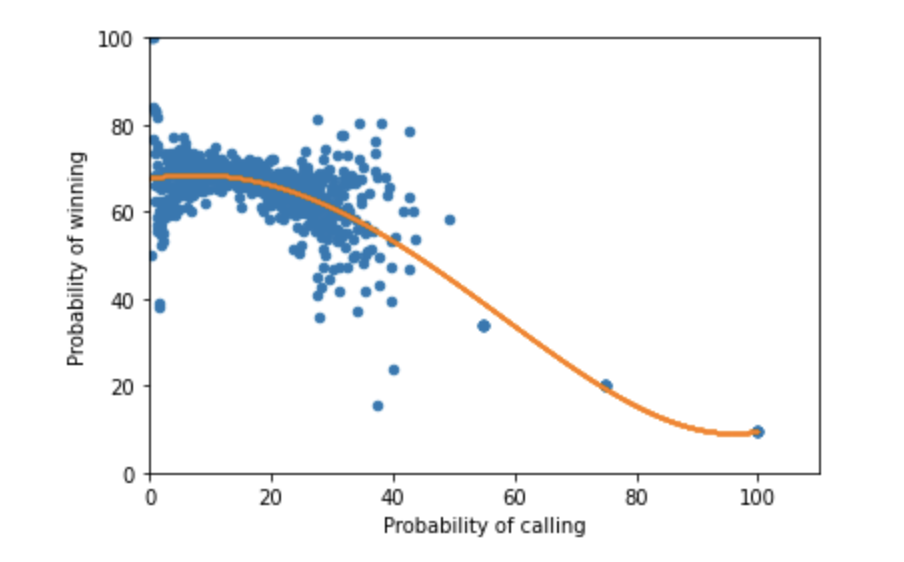
\includegraphics[width=0.5\textwidth]{Bilder/calling_winning_graph}
    \caption{$f4(x)=5.21140286\cdot 10^{-10}\cdot x^5+  7.51385614\cdot 10^{-07}\cdot x^4+  1.69471455\cdot 10^{-06}\cdot x^3+ -1.64932045\cdot 10^{-02}\cdot x^2+2.48230296\cdot 10^{-01}\cdot x + 67.7185027$}
    \label{fig:meine-grafik}
\end{figure}
The average probability for the double victory is calculated from the average of all players. So total number of doubles / total number of rounds.
\section{Simulation}
\subsection{B.1}
First of all, we will have a look on the outcome of the Exchange Stage under different circumstances. But which outcome is the best for a team? We try to get a maximal value in three different ways:

\paragraph{Maximum}  We are only looking at the card value of the higher cards, because this can lead to a win of Tichu
\paragraph{Square Addition}  We sum the squares of both card values, because it doesn’t look only at the higher card value and consider both card values of the team.
\paragraph{Square Diffrence} We take the difference of the squares of both card values and try to minimize it, because it can be good to have balanced players. 
\\
\\
We try to find the nash equilibrium in all three cases and set $\beta = 0$. The players will not know which strategies the other players follow. We will only look at case $\beta = 0$ for case 1, because the information on his partners strategy will only create a bigger difference but will result in the same tactics. 

To determine the nash equilibrium, we will use the average values, including $\lambda_ji = 0$ for opponents. So we only look at the partner exchange with X = 0.5, $\mu = \frac{1}{14}$, $\sigma = \frac{1}{28}$.

We will show the average card values with $\beta =0$. The actual payoffs can differ:
\begin{table}[h]
\resizebox{0.5\textwidth}{!}{%
\begin{tabular}{|c|c|c|}
\hline 
Receiving $\backslash$ Passing & A & D \\ 
\hline 
A & 0.5, 0.5 & $0.5+\frac{1}{14}$, $0.5-\frac{1}{14}$\\ 
\hline 
D & $0.5-\frac{1}{14}$, $0.5+\frac{1}{14}$ & 0.5, 0.5 \\
\hline 
\end{tabular}%
}
\end{table}

1. Maximum:
\begin{table}[h]
\resizebox{0.5\textwidth}{!}{%
\begin{tabular}{|c|c|c|}
\hline 
Receiving $\backslash$ Passing & A & D \\ 
\hline 
A & 0.5, 0.5 & $0.5+\frac{1}{14}$, $0.5+\frac{1}{14}$\\ 
\hline 
D & $0.5+\frac{1}{14}$, $0.5+\frac{1}{14}$ & 0.5, 0.5 \\
\hline 
\end{tabular}%
}
\end{table}

2. Square Addition:
\begin{table}[h]
\resizebox{0.5\textwidth}{!}{%
\begin{tabular}{|c|c|c|}
\hline 
Receiving $\backslash$ Passing & A & D \\ 
\hline 
A & 0.5, 0.5 & $\frac{25}{49}$, $\frac{25}{49}$\\ 
\hline 
D & $\frac{25}{49}$, $\frac{25}{49}$ & 0.5, 0.5 \\
\hline 
\end{tabular}%
}
\end{table}

Assuming, Player 1 is playing strategy A with a probability of p, we will find the mixed nash-equilibrium p = 0.5, q = 0.5 if Player 2 is playing with a probability of q:

\begin{figure}[!ht]
    \centering
    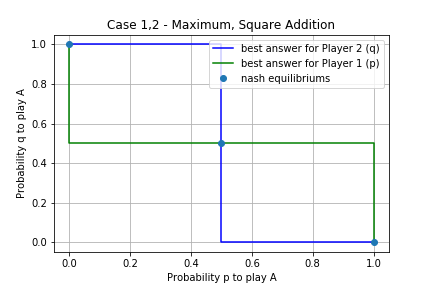
\includegraphics[width=0.5\textwidth]{Bilder/5_max}
    \caption{Case 1,2 - Maximum, Square Addition}
    \label{fig:meine-grafik}
\end{figure}

Anologously we can find the nash equilibrium for the third case.

3. Square Diffrence:

\resizebox{0.5\textwidth}{!}{%
\begin{tabular}{|c|c|c|}
\hline 
Receiving $\backslash$ Passing & A & D \\ 
\hline 
A & 0.0, 0.0 & $-\frac{1}{7}, \frac{1}{7}$ \\ 
\hline 
D & $-\frac{1}{7}, \frac{1}{7}$ & 0.0, 0.0 \\ 
\hline 
\end{tabular}%
}
\begin{figure}[!ht]
    \centering
    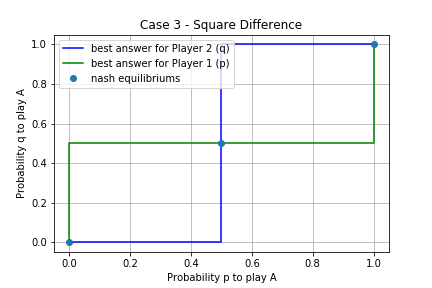
\includegraphics[width=0.5\textwidth]{Bilder/5_diff}
    \caption{Case 3 - Square Diffrence}
    \label{fig:meine-grafik}
\end{figure}

\subsubsection{Adjusting $\beta$}

If we set $\beta = 0$, we will only redefine the values, but the nash equilibrium will stay the same. Just from the cards, it is the best to play a mixed strategy for all cases. To enable this strategy in our simulation, we will now allow $\alpha$ to be in [0,1]. This will give us a well defined Exchange function as described before.

We always used $\beta$ as a fixed value in $\{0,1\}$. But in a real game, players can recognize the strategy of another player if they play enough games. Taking this into account, we will adjust $\beta$ during the game after each round. We decided to simulate the growth of knowledge with a logistic function, this is, in our point of view, the most realistix approximation of $\beta$ as at the beginning the growth of your information on other players is slowly but after some amount of games it speeded up. At the beginning, a Player has some information on the other players strategies (or does not). This value will be $\beta^{(0)}_{P}\in\{0,1\}$ for each Player $P\in\{1,2,3,4\}$. Note that now the knowledge of diffrent players $P_i\neq P_j$ can differ and develop throughout the game in diffrent ways based on the information given before the game. The player can get more information during the game. If he has much information, he will need more rounds to get new information on the other players. We will adjust this value to $\beta^{(1)}_{P}$ for the first round. This notation will lead us to the following adjusting, which will be described later on:
\begin{align*}
\beta^{(r+1)}_{P} = \frac{\beta^{(r)}_{P}
}{\beta^{(r)}_{P} + (1 - \beta^{(r)}_{P})} \cdot e^{-k}
\end{align*}
Where $k$ is in $\mathbb{R}_{>0}$ and $r$ is the number of rounds played. If $k$ is low, Players will learn slowly about other players strategies. If k is high, this process will be faster. We will now use $k = 0.2$, because we believe it is the most realistic function for $\beta$. An average round has <20 games and a knowledge of $80\%$ is way to high, while $10\%$ is low (see Chart):

\begin{figure}[h!]
    \centering
    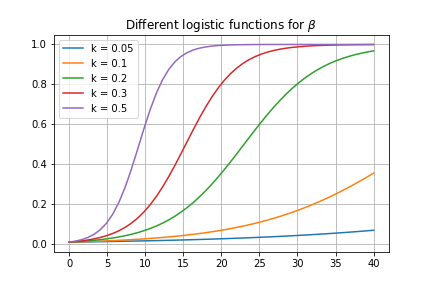
\includegraphics[width=0.5\textwidth]{Bilder/5_log}
    \caption{Adjusting $k$ for $\beta^{(r)}_{P}$}
    \label{fig:meine-grafik}
\end{figure}

\section{Conclusion}
At this point we would like to discuss our errors and approximations in the model and explore further possibilities for improvement.

\subsubsection{Subgame B.0}

Here is probably the most essential approximation that the Great Tichu was neglected. This is of course essential for the scuffing, because it makes the scuffing much clearer. Each team partner (with Common Knowledge) would then give his team mate a very good card, because he himself can and needs no more Tichu. At the same time, the opponents will try to get the worst possible cards, like the dog that doesn't fit into any combination. Also the card 1 is usually nudged by the opponents in such a way that the player who has announced the Great Tichu comes second and thus must react to the request.
Problems could also result from normal distributions etc. Even if these were chosen sensibly, they do not always reflect reality very well. Calculating the values of cards based on their combination is extremely difficult, since the time course of the game also influences the value of a combination.

\subsubsection{Subgame B.1}

Basically this part has a very theoretical basis. There are of course more possibilities to change parameters and to cover different cases to get a better evaluation.
But even here, a certain arbitrariness is sometimes found in the eta and xi function, for example, but the result is meaningful, as can be seen at the Nash equilibrium. This could of course be further improved with certain calculations and statistical surveys.

\subsubsection{Subgame B.2}

The model has of course been simplified at one point or another.
First we start with the player model. It is of course very difficult to map a player type exactly. The division into 3 types is of course not small enough to reflect reality. Above all, the increase in risk will also depend on the type of player. Although the basic aggressiveness was taken as the underlying, the increase was calculated independently. But it is precisely the different situations that will provoke different human reactions. Even if the average of the survey showed this, it may be different for individuals.
Also the assumption of common knowledge will not apply to every player in every situation. For once we have also used this assumption to eradicate certain situations and not have to take them into account.
For example, we said that if a Tichu from Team 1 and Team 2 is announced, one of the two teams will win in any case. But it is also possible that a third player wins this Tichu and this without violating the assumption of common knowledge.
The irrational behaviour could occur for various reasons.
An example would be a player's lack of experience. After all, you cannot conclude with 100% certainty from your own cards that you are superior to your opponents.
The experience gained also goes hand in hand with certain strategies. For example, the convention that one shuffles an even card to the right and an odd card to the left. This is very useful, provided that both team members adhere to it. But it cannot be interpreted as Common Knowledge, because right even and left odd was chosen arbitrarily and would make sense as well, if it was swapped.
Another component that we have neglected is the timing of the game. By waiting for certain tricks, one can exclude that certain cards are still in the game and thus increase the probability for an own Tichu if necessary. However, this was not taken into account in this case.
One possible technical error is, for example, the interpolation of data from the onlinetichu.com website. Various errors can occur, especially during interpolation.


Especially since little or no data is provided for higher announcement rates, for example.
In the future, it would be possible to work on all these points in order to improve the model further.

\end{document}

